\section{Технологический раздел}

\subsection{Реализация алгоритмов}

В листинге~\ref{des} представлен код алгоритма шифрования и дешифрования.

\begin{lstlisting}[label=des,caption=Исходный код шифрования, language=C]
void aes_encrypt(const uint8_t *in, uint8_t *out, uint8_t *key) {
    uint8_t state[WORD_SIZE * N_B];
    block_to_state(in, state);

    uint8_t expanded_key[WORD_SIZE * N_B * (N_R + 1)];
    expand_key(key, expanded_key);
    add_round_key(state, expanded_key, 0);

    for (uint8_t r = 1; r < N_R; r++) {
        sub_bytes(state);
        shift_rows(state);
        mix_columns(state);
        add_round_key(state, expanded_key, r);
    }

    sub_bytes(state);
    shift_rows(state);
    add_round_key(state, expanded_key, N_R);

    block_from_state(state, out);
}
\end{lstlisting}

\newpage
В листинге~\ref{des1} представлена реализация режима шифрования OBF.

\begin{lstlisting}[language=C, caption=Реализация режима шифрования OBF, label=des1]
void ofb(uint8_t *data, int num_blocks, uint8_t *iv, uint8_t *key) {
    uint8_t iv_copy[BLOCK_SIZE + 1];

    memcpy(iv_copy, iv, BLOCK_SIZE + 1);

    for (int i = 0; i < num_blocks; i++) {
        aes_encrypt(iv_copy, iv_copy, key);

        for (int j = 0; j < BLOCK_SIZE; j++) {
            data[BLOCK_SIZE * i + j] = data[BLOCK_SIZE * i + j] ^ iv_copy[j];
        }
    }
}
\end{lstlisting}	


\subsection{Тестирование}
\textbf{Входные данные}: имя входного файла, имя выходного файла, режим работы программы, ключ, начальный вектор.

\textbf{Выходные данные}: зашифрованный или расшифрованный файл в зависимости от режима работы программы.

Тестирование было проведено на файлах с типами: текстовый (txt), графический (bmp, png), архив (zip), несуществующий (ubc). Также, был проведен тест с повреждением зашифрованного файла.

В таблице \ref{tbl:test} представлены тестовые данные.

\begin{table}[H]
	\begin{center}
		\centering
		\caption{Тестовые данные}
		\label{tbl:test}
		\begin{tabular}{|c|c|c|} 
			
			\hline
			\multicolumn{1}{|c|}{Номер теста}
			&  \multicolumn{1}{c|}{Тип файла} &  \multicolumn{1}{c|}{Содержимое файла}\\
			\hline
			
			1& txt &  {\specialcell{Наглая Пугачева}} \\ \hline
			
			2& ubc &  $\varnothing$\\ \hline
			
			3& zip & Файлы с тестов 1, 2, 4 \\ \hline
			
			4& png & {\specialcell{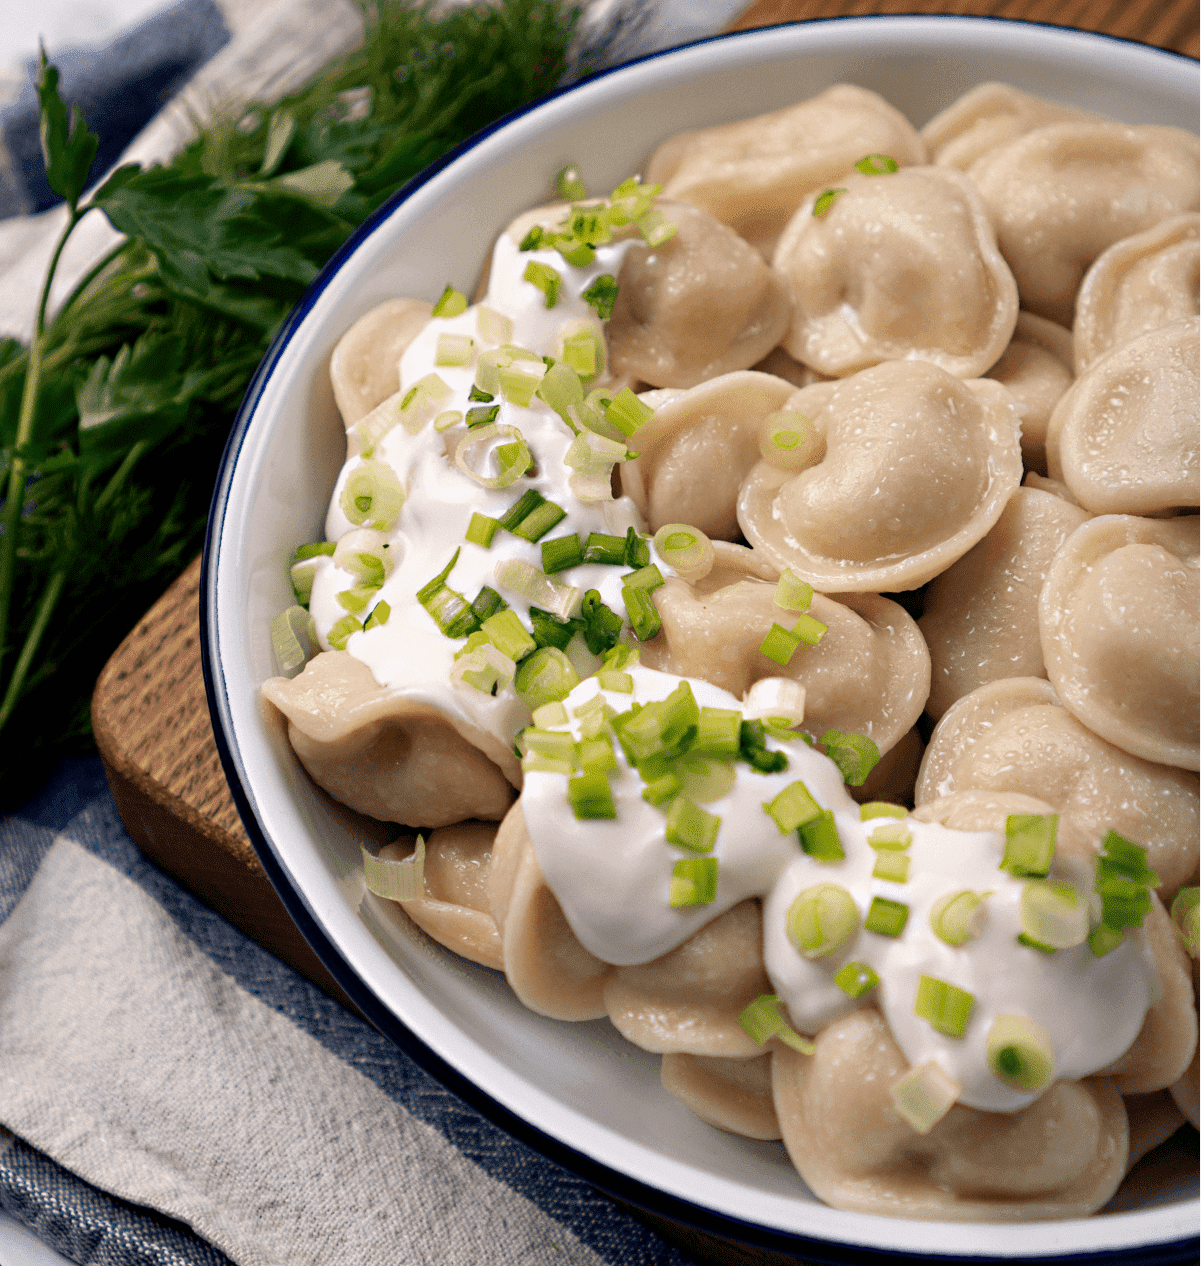
\includegraphics[width=1in]{assets/test4.png}}} \\ \hline
			
			5& bmp & {\specialcell{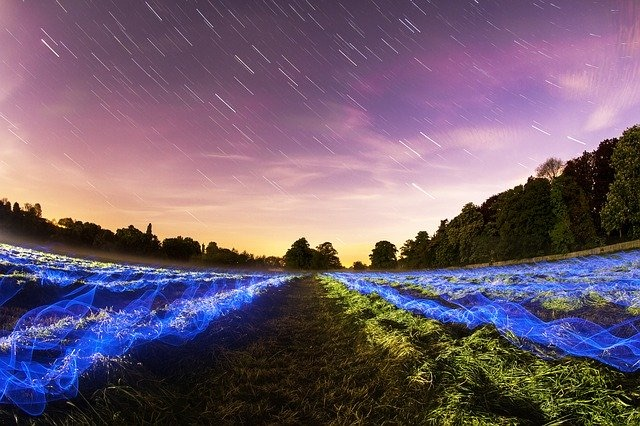
\includegraphics[width=1in]{assets/test7.jpeg}}} \\ \hline
			
			6& {\specialcell{bmp (corrupted)\\(in english)}} & {\specialcell{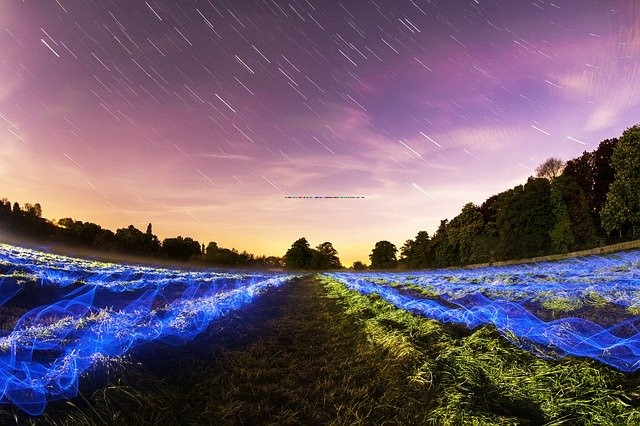
\includegraphics[width=1in]{assets/test7.dec.jpeg}}} \\ \hline
			
		\end{tabular}
	\end{center}
\end{table}


\newpage